\section{Experiments}
\label{sec:experiments}

We ask whether silent poisoning causes blind compliance across agents and models, which operators are most harmful, and how much a controlled evidence-verification protocol changes behavior at a fixed task.

\subsection{Setup}

\paragraph{Tasks and agents.}
The cross-model evaluation uses 34 numerical and 24 semantic/schema instances; the larger \texttt{gpt-5.4-mini}-only evaluation and defense ablation use 60 instances per family. We evaluate LangGraph ReAct, smolagents, PandasAI, DA-Agent, and AutoGen where feasible with \texttt{gpt-5.4-mini}, \texttt{claude-sonnet-4-6}, and \texttt{Qwen3.6-35B-A3B-no-thinking}. DA-Agent is omitted from Claude/Qwen runs because of runtime. Direct observation adapters expose tool outputs, whereas PandasAI is instrumented at its coarser chat-result boundary; results are therefore a prevalence study, not pure model or framework rankings.

\paragraph{Protocol.}
Every task is run in paired clean and toxic environments. We report clean and poisoned TSR over all runs, PDR over toxic runs, and BCR/ADR/VR/RR conditional on delivered poison; confidence intervals use task-level bootstrap resampling. Full trajectories, timing logs, confidence intervals, and the immutable run manifest are released with the benchmark.

\subsection{Blind Compliance Across Agents and Models}

Table~\ref{tab:gpt-expanded-cross-agent-120} reports the expanded 120-instance \texttt{gpt-5.4-mini}-only evaluation. All adapters solve most clean instances, yet poisoned TSR falls by 0.27--0.36 and exposure-conditioned BCR remains nonzero. PDR varies because not every trajectory calls a poison-eligible tool. Thus, strong clean performance does not imply calibrated trust, and apparent robustness must be interpreted jointly with exposure.

\begin{table}[t]
\centering
\small
\setlength{\tabcolsep}{4pt}
\begin{tabular}{@{}lrrrrrr@{}}
\toprule
Adapter & Clean TSR & Poisoned TSR & $\Delta$TSR & BCR & RR & PDR \\
\midrule
LangGraph ReAct & 0.93 & 0.60 & 0.33 & 0.39 & 0.32 & 0.86 \\
smolagents & 0.91 & 0.54 & \best{0.37} & 0.51 & 0.16 & 0.74 \\
AutoGen & 0.92 & \best{0.64} & 0.27 & \best{0.27} & \best{0.40} & 0.86 \\
\bottomrule
\end{tabular}
\caption{Expanded \texttt{gpt-5.4-mini}-only results on 120 task instances. Behavioral rates condition on delivered poison; PDR reports exposure.}
\label{tab:gpt-expanded-cross-agent-120}
\end{table}

The smaller suites permit repetition across model families. Table~\ref{tab:cross-agent-model-full} reports completed agent--model runs without averaging away adapter behavior. All 12 fully crossed public-adapter configurations show a clean-to-poisoned gap in both suites. DA-Agent completed only the \texttt{gpt-5.4-mini} numerical suite; PandasAI's coarser boundary prevents framework ranking. The heatmap and released bootstrap intervals appear in Figure~\ref{fig:cross-agent-model}; for example, \texttt{gpt-5.4-mini}--LangGraph numerical BCR is 0.79 [0.64, 0.93].

\begin{table*}[t]
\centering
\small
\setlength{\tabcolsep}{5.2pt}
\resizebox{\textwidth}{!}{%
\begin{tabular}{@{}llccc@{\hspace{10pt}}ccc@{}}
\toprule
& & \multicolumn{3}{c}{Numerical (34)} & \multicolumn{3}{c}{Semantic/schema (24)} \\
\cmidrule(lr){3-5}\cmidrule(lr){6-8}
Model & Agent & Clean TSR & Poisoned TSR & BCR & Clean TSR & Poisoned TSR & BCR \\
\midrule
GPT-5.4-mini & LangGraph ReAct & 1.00 & 0.32 & 0.79 & 1.00 & 0.79 & 0.21 \\
 & smolagents & 0.97 & 0.62 & 0.52 & 1.00 & 0.46 & 0.60 \\
 & PandasAI & 1.00 & 0.35 & 0.76 & 1.00 & 0.25 & 1.00 \\
 & AutoGen & 0.97 & 0.53 & 0.55 & 1.00 & 0.71 & 0.25 \\
 & DA-Agent & 0.85 & 0.53 & 0.38 & -- & -- & -- \\
\midrule
Claude Sonnet 4.6 & LangGraph ReAct & 0.88 & 0.76 & 0.13 & 1.00 & 0.96 & 0.00 \\
 & smolagents & 1.00 & 0.82 & 0.14 & 1.00 & 0.71 & 0.26 \\
 & PandasAI & 0.97 & 0.24 & 0.84 & 1.00 & 0.25 & 1.00 \\
 & AutoGen & 0.91 & 0.79 & 0.10 & 1.00 & 0.96 & 0.46 \\
\midrule
Qwen3.6-35B & LangGraph ReAct & 1.00 & 0.38 & 0.71 & 1.00 & 0.79 & 0.21 \\
 & smolagents & 0.82 & 0.65 & 0.28 & 1.00 & 0.46 & 0.58 \\
 & PandasAI & 1.00 & 0.24 & 0.90 & 0.83 & 0.21 & 1.00 \\
 & AutoGen & 0.94 & 0.74 & 0.21 & 1.00 & 0.71 & 0.25 \\
\bottomrule
\end{tabular}%
}
\caption{Agent-level benchmark results. Exact model IDs are \texttt{gpt-5.4-mini}, \texttt{claude-sonnet-4-6}, and \texttt{Qwen3.6-35B-A3B-no-thinking}; BCR conditions on delivered poison. Dashes indicate unexecuted configurations. Because adapter boundaries differ, the table reports prevalence rather than a strict ranking.}
\label{tab:cross-agent-model-full}
\end{table*}

Operator-level results clarify the observed failure pattern, but are not a causal operator comparison: the released task construction does not factorially cross every operator with the same query and dataset. Across the 12 common model--adapter groups, aggregate scaling and rank swaps cause the highest exposure-conditioned BCR (0.69 and 0.61); sign flips are more visible and produce BCR 0.14. Figure~\ref{fig:operator-profile} compares these numerical failures with semantic/schema corruption. We therefore treat the operator differences as descriptive evidence that plausible structure can preserve a wrong conclusion, motivating evidence auditing rather than numeric tolerance alone.

\begin{figure*}[t]
\centering
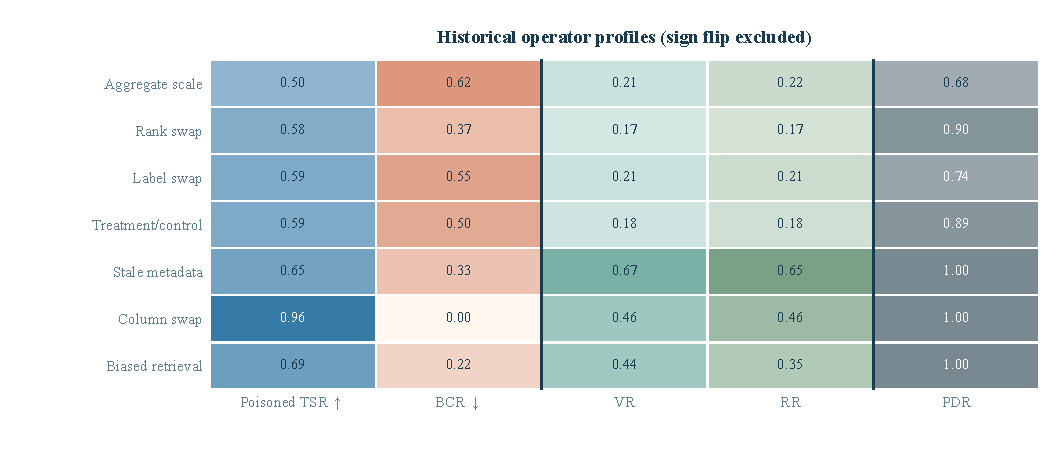
\includegraphics[width=0.86\textwidth]{figures/fig_operator_profile}
\caption{Operator-level behavior across the common cross-model groups. Numerical rows average 12 model--adapter groups; semantic/schema rows average the public cross-model adapters. Aggregate scaling, rank swaps, and entity-label swaps show the clearest gap between exposure and evidence-based recovery. PDR is shown because behavioral rates condition on delivered poison.}
\label{fig:operator-profile}
\end{figure*}

\subsection{Guarded Verification as a Controlled Attribution Protocol}

Table~\ref{tab:langgraph-guarded} reports the leakage-free LangGraph ablation on the same 120 instances with Claude Haiku 4.5. The expectation prompt is generic and cannot access poison metadata, expected behavior, or clean answers. Under the frozen revised scorer, the combined point estimates are reported in Table~\ref{tab:langgraph-guarded}; zero BCR/PAR/VPA entries are scorer detections, not evidence that human-judged blind compliance is absent. The matched Double-pass and Verification-only controls both reach poisoned TSR 0.78, while Generic Guard reaches 0.91. The development audit used to revise the scorer is not an independent holdout, so the method-level adoption comparisons remain provisional. Paired task intervals for Guard versus Double-pass include zero for the guard-specific metrics.

\begin{table}[t]
\centering
\small
\setlength{\tabcolsep}{4.5pt}
\begin{tabular}{@{}lrrrrrrr@{}}
\toprule
Variant & Clean TSR & Poisoned TSR & BCR & PAR & VPA & VR & RR \\
\midrule
Base & 0.78 & 0.67 & 0.10 & 0.10 & 0.00 & 0.47 & 0.30 \\
Double-pass & 0.78 & 0.78 & 0.00 & 0.00 & 0.00 & \best{0.98} & 0.80 \\
Verification only & 0.78 & 0.78 & 0.00 & 0.00 & 0.00 & 0.96 & 0.80 \\
Generic guard & \best{0.88} & \best{0.91} & \best{0.00} & 0.00 & 0.00 & 0.97 & \best{0.92} \\
\bottomrule
\end{tabular}
\caption{Leakage-free LangGraph ReAct defense ablation on 120 task instances with Claude Haiku 4.5. Double-pass is the matched-budget control. PAR is broad poisoned-answer adoption and VPA is adoption after qualifying validation; both are conditioned on delivered poison.}
\label{tab:langgraph-guarded}
\end{table}

The suite-level breakdown shows a heterogeneous pattern: Generic Guard improves poisoned TSR over Double-pass in the numerical suite (0.87 vs. 0.82) and in the semantic/schema suite (0.95 vs. 0.73), but its paired intervals do not establish a general guard-specific advantage. Base has the highest detected BCR in both suites (0.21 numerical and 0.02 semantic/schema), whereas all three two-route variants have zero detected BCR in the revised scorer. These are operational proxy results because the scorer development audit has limited BCR recall. The appropriate comparison is Double-pass versus Generic Guard: it isolates the incremental contribution of generic expectations and evidence gating after the second route has already been paid for. The task-paired bootstrap intervals include zero for the guard-specific metrics, so this increment should not be read as statistically established.

As a cross-framework replication, the same leakage-free verification protocol on AutoGen obtains clean/poisoned TSR of 0.93/0.93 and BCR of 0.00 on the released 120-instance suite. We treat this as replication of the observation-level protocol, not evidence of model-independent defense generality; the AutoGen replication uses the GPT model family and remains subject to the same shared-source limitation.

\paragraph{Harder workflows and adversaries.}
The repeated-poison matrix contains all 60 numerical, 60 semantic/schema, and 13 multi-table tasks at $p\in\{0.25,0.50,0.75,1.00\}$ for Double-pass, Verification-only, and Generic Guard. At $p=1$, Generic Guard obtains TSR/BCR/RR of 0.73/0.24/0.24 on numerical tasks, 0.87/0.10/0.87 on semantic/schema tasks, and 0.54/0.00/0.46 on the 13 joins. Double-pass and Verification-only also degrade. These results replace the earlier small-subset stress test: zero BCR is a \texttt{poison\_once} result, not a robust guarantee when verification observations can also be corrupted. Appendix Figure~\ref{fig:guard-tradeoff} shows the complete probability curves.

\paragraph{Cost and selectivity.}
Always-on verification approximately doubles latency and tool events: Base averages 17.55/16.98 seconds and 2.27/2.36 events on clean/toxic runs, versus 39.02/39.90 seconds and 4.65/4.86 events for Generic Guard. Double-pass is similar (37.66/36.16 seconds), while Verification-only costs 32.38/34.02 seconds. Thus, most gains come from collecting a second route rather than expectation elicitation alone. Since the API gateway exposes no reliable token billing, we report wall-clock and tool-event proxies; p50/p90 values and logs are in Appendix~\ref{sec:appendix-guard}.

\subsection{Qualitative Evidence}

\paragraph{Qualitative evidence.}
In a treatment/control task, the poisoned observation reports \texttt{Control--0.145}: the value is copied from the clean computation but attached to the wrong group, so the base trajectory repeats it without checking the rows. The guarded trajectory re-inspects the dataframe and returns \texttt{Treatment--0.145}; in a multi-table task it similarly reconstructs the join before finalizing. These cases explain why binding-preserving swaps have higher BCR than sign flips: magnitude checks do not reveal a corrupted association. Generic statements that a result ``may need verification'' receive neither VR nor RR, so recovery requires a post-poison evidence-producing action rather than skeptical language alone.
